\chapter{Ein Anhang}
...falls gewünscht...

Und hier noch ein Text aus dem Projekt Gutenberg zum Test der Ränder und des optischen Randausgleichs

Des Lebens Überfluss\footnote{\url{http://gutenberg.spiegel.de/tieck/ueberflu/ueberflu.htm}} von Ludwig Tieck.

In einem der härtesten Winter war gegen Ende des Februar ein sonderbarer Tumult gewesen, über dessen Entstehung, Fortgang und Beruhigung die seltsamsten und widersprechendsten Gerüchte in der Residenz umliefen. Es ist natürlich, dass, wenn alle Menschen sprechen und erzählen wollen, ohne den Gegenstand ihrer Darstellung zu kennen, auch das Gewöhnliche die Farbe der Fabel annimmt.

In der Vorstadt, die ziemlich bevölkert ist hatte sich in einer der engsten Straßen das Abenteuer zugetragen. Bald hieß es, ein Verräter und Rebell sei entdeckt und von der Polizei aufgehoben worden, bald, ein Gottesleugner, der mit andern Atheisten verbrüdert das Christentum mit seiner Wurzel ausrotten wollen, habe sich nach hartnäckigem Widerstand den Behörden ergeben und sitze nun so lange fest, bis er in der Einsamkeit bessere Grundsätze und Überzeugungen finde. Er habe sich aber vorher noch in seiner Wohnung mit alten Doppelhaken, ja sogar mit einer Kanone verteidigt, und es sei, bevor er sich ergeben, Blut geflossen, so dass das Konsistorium wie das Kriminalgericht wohl auf seine Hinrichtung antragen werde. Ein politischer Schuhmacher wollte wissen, der Verhaftete sei ein Emissär, der als das Haupt vieler geheimen Gesellschaften mit allen Revolutionsmännern Europas in innigster Verbindung stehe; er habe alle Fäden in Paris, London und Spanien wie in den östlichen Provinzen gelenkt, und es sei nahe daran, dass im äußersten Indien eine ungeheure Empörung ausbrechen und sich dann gleich Cholera nach Europa herüberwälzen werde, um allen Brennstoff in lichte Flammen zu setzen.

So viel war ausgemacht, in einem kleinen Hause hatte es Tumult gegeben, die Polizei war herbeigerufen worden, das Volk hatte gelärmt, angesehene Männer wurden bemerkt, die sich darein mischten, und nach einiger zeit war alles wieder ruhig, ohne dass man den Zusammenhang begriff. Im Hause selbst war eine gewisse Zerstörung nicht zu verkennen. Jeder legte sich die Sache aus, wie Laune oder Phantasie sie ihm erklären mochten. Die Zimmerleute und Tischler besserten nachher den Schaden aus.

Ein Mann hatte in diesem Hause gewohnt, den niemand in der Nachbarschaft kannte. War er ein Gelehrter? ein Politiker? ein Einheimischer? ein Fremder? Darüber wusste keiner, selbst der Klügste nicht, einen genügenden Bescheid zu geben.

Soviel ist gewiss, dieser unbekannte Mann lebte sehr still und eingezogen, man sah ihn auf keinem Spaziergange, an keinem öffentlichen Orte. Er war noch nicht alt, wohlgebildet, und seine junge Frau, die sich mit ihm dieser Einsamkeit ergeben hatte, durfte man eine Schönheit nennen.

Um Weihnachten war es, als dieser jugendliche Mann in seinem Stübchen, dicht am Ofen sitzend, also zu seiner Frau redete: »Du weißt, liebste Klara, wie sehr ich den Siebenkäs unsers Jean Paul liebe und verehre; wie dieser sein Humorist sich aber helfen würde, wenn er in unsrer Lage wäre, bleibt mir doch ein Rätsel. Nicht wahr, Liebchen, jetzt sind, so scheint es, alle Mittel erschöpft?«

»Gewiss, Heinrich«, antwortete sie lächelnd und zugleich seufzend; »wenn du aber froh und heiter bleibst, liebster aller Menschen, so kann ich mich in deiner Nähe nicht unglücklich fühlen.«

»Unglück und Glück sind nur leere Worte«, antwortete Heinrich; »als du mir aus dem Hause deiner Eltern folgtest, als du so großmütig um meinetwillen alle Rücksichten fahren ließest: da war unser Schicksal auf unsre Lebenszeit bestimmt. Lieben und leben hieß nun unsre Losung; wie wir leben würden, durfte uns ganz gleichgültig sein. Und so möchte ich noch jetzt aus starkem Herzen fragen: Wer in ganz Europa ist wohl so glücklich, als ich mich mit vollem Recht aus der ganzen Kraft meines Gefühles nennen darf?«

»Wir entbehren fast alles«, sagte sie, »nur uns selbst nicht, und ich wusste ja, als ich den Bund mit dir schloss, dass du nicht reich warst; dir war es nicht unbekannt, dass ich aus meinem väterlichen Hause nichts mit mir nehmen konnte. So ist die Armut mit unsrer Liebe eins geworden, und dieses Stübchen, unser Gespräch, unser Anblicken und Schauen in des Geliebten Auge ist unser Leben.«

»Richtig!« rief Heinrich aus und sprang auf in seiner Freude, um die Schöne lebhaft zu umarmen; »wie gestört, ewig getrennt, einsam und zerstreut wären wir nun in jenem Schwarm der vornehmen Zirkel, wenn alles in seiner Ordnung vor sich gegangen wäre. Welch Blicken, Sprechen, Handgeben, Denken dort! Man könnte sich Tiere oder selbst Marionetten so abrichten und eindrechseln, dass sie eben die Komplimente machten und solche Redensarten von sich gäben. So sind wir, mein Schatz, wie Adam und Eva hier in unserm Paradiese, und kein Engel kommt auf den ganz überflüssigen Einfall, uns daraus zu vertreiben.«

»Nur«, sagte sie etwas kleinlaut, »fängt das Holz an, ganz einzugehen, und dieser Winter ist der härteste, den ich bis jetzt noch erlebt habe.«

Heinrich lachte. »Sieh«, rief er, »ich muss aus purer Bosheit lachen, aber es ist darum noch nicht das Lachen der Verzweiflung, sondern einer gewissen Verlegenheit, da ich durchaus nicht weiß, wo ich Geld hernehmen könnte. Aber finden müssen sich die Mittel; denn es ist undenkbar, dass wir erfrieren sollten, bei so heißer Liebe, bei so warmem Blut! Pur unmöglich!«

Sie lachte ihn freundlich an und erwiderte: »Wenn ich nur so wie Lenette Kleider zum Verkaufe mitgebracht, oder überflüssige Messingkannen und Mörser oder kupferne Kessel in unsrer kleinen Wirtschaft umherständen, so wäre leicht Rat zu finden.«

»Jawohl«, sprach er mit übermütigem Ton, »wenn wir Millionärs wären, wie jener Siebenkäs, dann wäre es keine Kunst, Holz anzuschaffen und selbst bessere Nahrung.«

Sie sah im Ofen nach, in welchem Brot in Wasser kochte, um so das kärglichste Mittagsmahl herzustellen, welches dann mit einem Nachtisch von weniger Butter beschlossen werden sollte. »Während du«, sagte Heinrich, »die Aufsicht über unsre Küche führst und dem Koch die nötigen Befehle erteilst, werde ich mich zu meinen Studien niedersetzen. Wie gern schriebe ich wieder, wenn mir nicht Tinte, Papier und Feder völlig ausgegangen wären; ich möchte auch wieder einmal etwas lesen, was es auch sei, wenn ich nur noch ein Buch hätte.«

»Du musst denken, Liebster«, sagte Klara und sah schalkhaft zu ihm hinüber; »die Gedanken sind dir hoffentlich noch nicht ausgegangen.«

»Liebste Ehefrau«, erwiderte er, »unsre Wirtschaft ist so weitläuftig und groß, dass sie wohl deine ganze Aufmerksamkeit in Anspruch nimmt; zerstreue dich ja nicht, damit nicht unsre ökonomischen Verhältnisse in Verwirrung geraten. Und da ich mich jetzt in meine Bibliothek begebe, so lass mich vor jetzt in Ruhe; denn ich muss meine Kenntnisse erweitern und meinem Geiste Nahrung gönnen.«

»Er ist einzig!« sagte die Frau zu sich selber und lachte fröhlich; »und wie schön er ist!«

»So lese ich denn wieder in meinem Tagebuche«, sprach Heinrich, »das ich ehemals anlegte, und es interessiert mich, rückwärts zu studieren, mit dem Ende anzufangen und mich so nach und nach zu dem Anfange vorzubereiten, damit ich diesen um so besser verstehe. Immer muss alles echte Wissen, alles Kunstwerk und gründliche Denken in einen Kreis zusammenschlagen und Anfang und Ende innigst vereinigen, wie die Schlange, die sich in den Schwanz beißt – ein Sinnbild der Ewigkeit, wie andre sagen; ein Symbol des Verstandes und alles Richtigen, wie ich behaupte.«

Er las auf der letzten Seite, aber nur halblaut: »Man hat ein Märchen, dass ein wütender Verbrecher, zum Hungertode verdammt, sich selber nach und nach aufspeiset; im Grunde ist das nur die Fabel des Lebens und eines jeden Menschen. Dort blieb am Ende nur der Magen und das Gebiss übrig, bei uns bleibt die Seele, wie sie das Unbegreifliche nennen. Ich aber habe mich abgestreift und abgelebt. Es war beinah lächerlich, dass ich noch einen Frack nebst Zubehör besaß, da ich niemals ausgehe. Am Geburtstage meiner Frau werde ich in Weste und Hemdärmeln vor ihr erscheinen, da es doch unschicklich wäre, bei hoffährigen Leuten in einem ziemlich abgetragenen Überrock Cour zu machen.«

»Hier geht die Seite und das Buch zu Ende«, sagte Heinrich. »Alle Welt sieht ein, dass unsre Fracks eine dumme und geschmacklose Kleidung sind, alle schelten diese Uniform, aber keiner macht, so wie ich, Ernst damit, den Plunder ganz abzuschaffen. Ich erfahre nun nicht einmal aus den Zeitungen, ob andere Denkende meinem kühnen Beispiele und Vorgange folgen werden.«

Er schlug um und las die vorige Seite: »Man kann auch ohne Servietten leben. Wenn ich bedenke, wie unsre Lebensweise immer mehr und mehr in Surrogat, Stellvertretung und Lückenbüßerei übergegangen ist, so bekomme ich einen rechten Hass auf unser geiziges und knickerndes Jahrhundert und fasse, da ich es ja haben kann, den Entschluss, in der Weise unsrer viel freigebigern Altvordern zu leben. Diese elenden Servietten sind ja, was selbst die heutigen Engländer noch wissen und verachten, offenbar nur erfunden, um das Tischtuch zu schonen. Ist es also Großmut, das Tischtuch nicht zu achten, so gehe ich darin noch weiter, das Tafeltuch zusamt den Servietten für überflüssig zu erklären. Beides wird verkauft, um vom saubern Tische selbst zu essen, nach Weise er Patriarchen, nach Art der – nun? welcher Völker? Gleichviel! Essen doch viele Menschen selbst ohne Tisch. Und, wie gesagt, ich treibe dergleichen nicht aus zynischer Sparsamkeit, nach Art des Diogenes, aus dem Hause, sondern im Gegenteil im Gefühl meines Wohlstandes, um nur nicht, wie die jetzige Zeit, aus törichtem Sparen zum Verschwender zu werden.«

»Du hast es getroffen«, sagte die Gattin lächeln; »aber damals lebten wir von dem Erlös dieser überflüssigen Sachen doch noch verschwenderisch. Oft sogar hatten wir zwei Schüsseln.«

Jetzt setzten sich die beiden Gatten zum dürftigsten Mahle nieder. Wer sie gesehen, hätte sie für beneidenswerte halten müssen, so fröhlich, ja ausgelassen waren sie an der einfachen Tafel. Als die Brotsuppe verzehrt war holte Klara mit schalkhafter Miene einen verdeckten Teller aus dem Ofen und setzte dem überraschten Gatten noch einige Kartoffeln vor. »Sieh!« rief dieser, »das heißt einem, wenn man sich an den vielen Büchern satt studiert hat, eine heimliche Freude machen! Dieser gute Erdapfel hat mit zu der großen Umwälzung von Europa beigetragen. Der Held Walter Raleigh soll leben!« – Sie stießen mit den Wassergläsern an, und Heinrich sah nach, ob der Enthusiasmus auch nicht einen Riss im Glase verursacht habe. »Um diese ungeheure Künstlichkeit«, sagte er dann, »um diese Einrichtung mit unsern alltäglichen Gläsern würden uns die reichsten Fürsten des Altertums beneidet haben. Es muss langweilig sein, aus einem goldenen Pokal zu trinken, vollends so schönes, klares, gesundes Wasser. Aber in unsern Gläsern schwebt die erfrischende Welle so heiter durchsichtig, so eins mit dem Becher, dass man wirklich versucht wird, zu glauben, man genieße den flüssig gewordenen Äther selbst. – Unsre Mahlzeit ist geschlossen; umarmen wir uns.«

\section{Weitere Illustrationen}
Abbildungen~\ref{fig:AnhangsChor} und~\ref{fig:AnhangsChor2} zeigen zwei Choreographien, die den
Sachverhalt weiter erläutern sollen. Die zweite Abbildung ist um 90 Grad gedreht, um das Paket
\texttt{rotating} zu demonstrieren.

\begin{figure}
  \begin{center}
    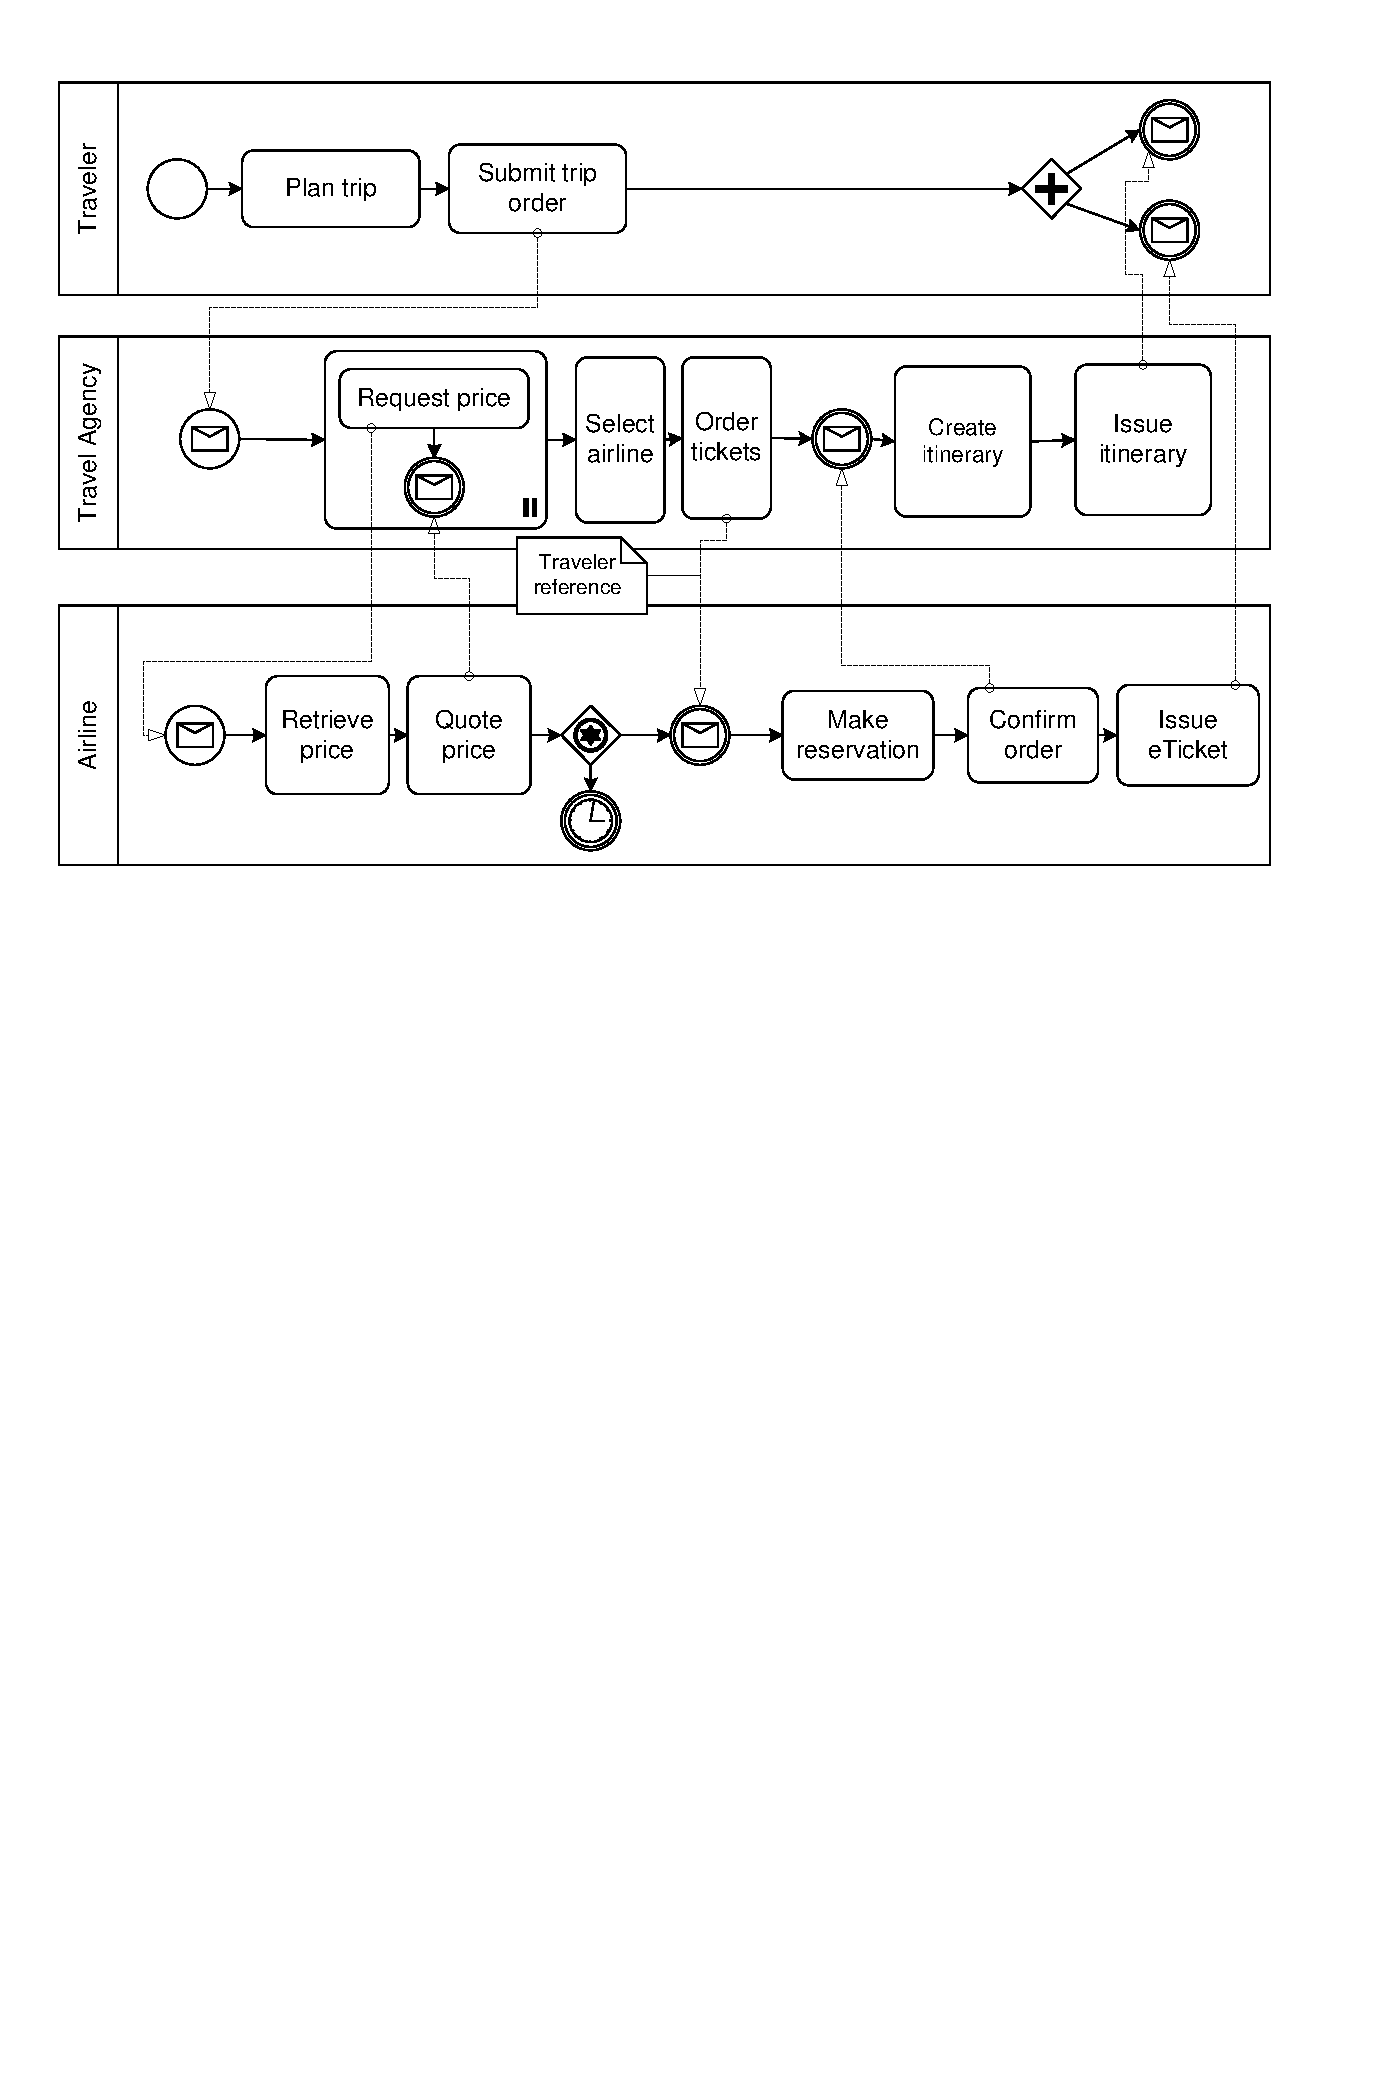
\includegraphics[width=\textwidth]{choreography.pdf}
    \caption{Beispiel-Choreographie I}
    \label{fig:AnhangsChor}
  \end{center}
\end{figure}

\begin{landscape}
%sidewaysfigure
\begin{figure}
  \begin{center}
    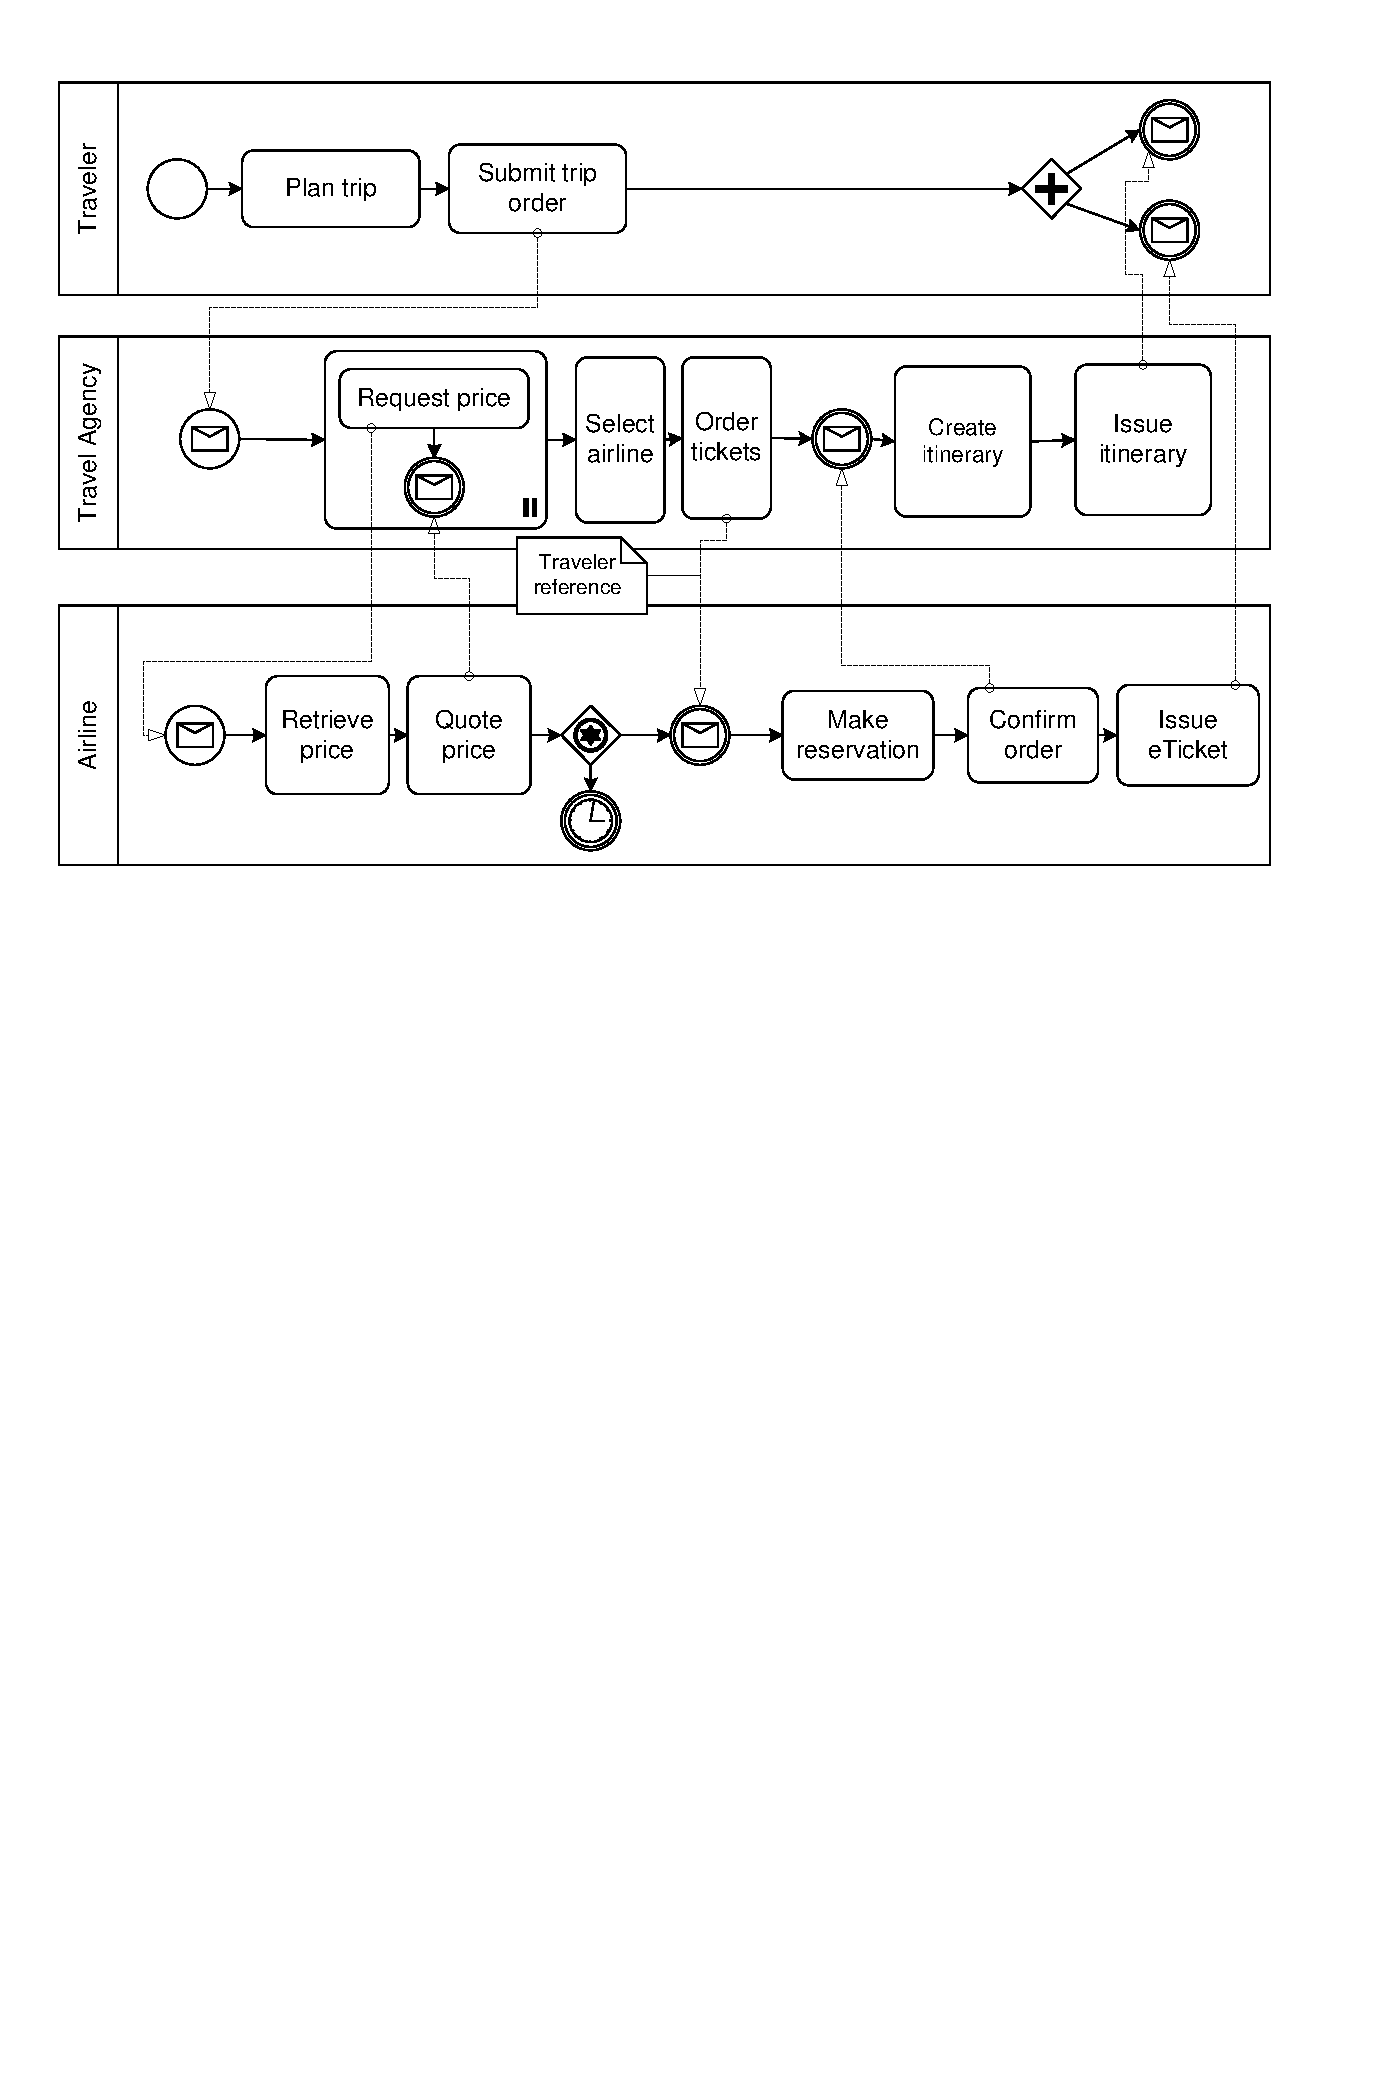
\includegraphics[width=\textwidth]{choreography.pdf}
    \caption{Beispiel-Choreographie II}
    \label{fig:AnhangsChor2}
  \end{center}
\end{figure}
\end{landscape}
